\begin{figure}[H]
	\begin{center}
		\begin{tikzpicture}[thick]
			\begin{scope}
				\path [draw=blue,snake arrow,->]
				(-4,0) -- (-2,0) node[anchor=south]{\hspace{-2cm}$h\nu$};
				\filldraw[black] (-1,0) circle (2pt) node[anchor=north]{$\vec e$};
			\end{scope}
			$\implies$
			\begin{scope}
				\path [draw=blue,dashed] (1,0)--(4,0);
				\path [draw=blue,snake arrow,->]
				(2,0) -- (3.5,1) node[anchor=east]{\hspace{-2cm}$h\nu'$};
				\path [draw=black, ->]
				(2,0) -- (2.5,-1) node[anchor=west]{$\vec p_e$};
				\draw[black] (3,0) arc (0:31:1) node[anchor=west]{$\theta$};
			\end{scope}
		\end{tikzpicture}
	\end{center}
	\caption{Комптон-эффект}
\end{figure}
\begin{figure}[H]
	\begin{center}
		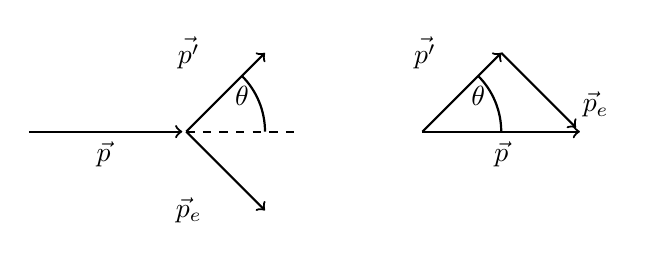
\begin{tikzpicture}[thick]
			\begin{scope}
				\path[draw=black,->] (-2,0)--(-0.05,0) node[anchor=north]{\hspace{-2cm}$\vec p$};
				\path[draw=black,->] (0,0)--(1,1) node[anchor=west]{\hspace{-2cm}$\vec {p'}$};
				\path[draw=black,->] (0,0)--(1,-1) node[anchor=west]{\hspace{-2cm}$\vec p_e$};
				\draw[black] (1,0) arc (0:45:1) node[anchor=north]{$\theta$};
				\path[draw=black,dashed] (0,0)--(1.4,0) ;
			\end{scope}
			%			$\Leftrightarrow$
			\begin{scope}
				\path[draw=black,->] (3,0)--(5,0) node[anchor=north]{\hspace{-2cm}$\vec p$};
				\path[draw=black,->] (3,0)--(4,1) node[anchor=west]{\hspace{-2cm}$\vec {p'}$};
				\path[draw=black,->] (4,1)--(4.95,0.05) node[anchor=south]{\hspace{0.5cm}$\vec p_e$};
				\draw[black] (4,0) arc (0:45:1) node[anchor=north]{$\theta$};
			\end{scope}
		\end{tikzpicture}
	\end{center}
	\caption{Закон сохранения импульса}
\end{figure}